\section{State-Of-The-Art}
In this section related work and literature on the topic is discussed.

\subsection{Related Work}
While there is some literature available on component-based architectures, I am not aware of works that researched
moving from an inheritance based approach to a component based approach on the same product. I think this is the first
work describing the actual process. I am also not aware of any case studies of \OS{} real-time strategy game
architectures and object representation.

\subsection{Literature}
A small number of papers and books on the topic is available:
\begin{enumerate}
    \item A Generic Framework for Game Development - \cite{Fh02ageneric}
    \item A Software Architecture for Games - \cite{Doherty_2003}
    \item A flexible and expandable architecture for computer games - \cite{Plummer_2004}
    \item Game Architecture and Design: A New Edition - \cite{Rollings.2003}
\end{enumerate}

Most literature titled component-based embraces the use of components in a high level view. They define a component
as a library of classes that fulfilles a certain functionality (such as physics, AI or rendering), whereas I am
interested in the low level component design, where a component maps to a single class of functionality.

\cite{Rollings.2003} seperates between a hard and soft architecture. The hard architecture is the part of the
architecture that is platfrom or domain specific, whereas the soft architecture is usually mostly the game-logic itself.
In \cite{springerlink:10.1007/978-3-540-73551-95} Folmer gives a "Reference Architecture" for games, which can be seen in
\figref{fig:referencearch}. The soft archticture described in \cite{Rollings.2003} is only the \textit{Game Interface}
and \textit{Domain Specific} layers in this reference architecture, the rest is considered hard architecture. I am
interested in the components of the \textit{Game Interface} layer of the of soft-architecture, whereas most
research is done on the broad topic of the hard architecture or the \textit{Domain Specific} layer.

\begin{figure}[!htb]
\center
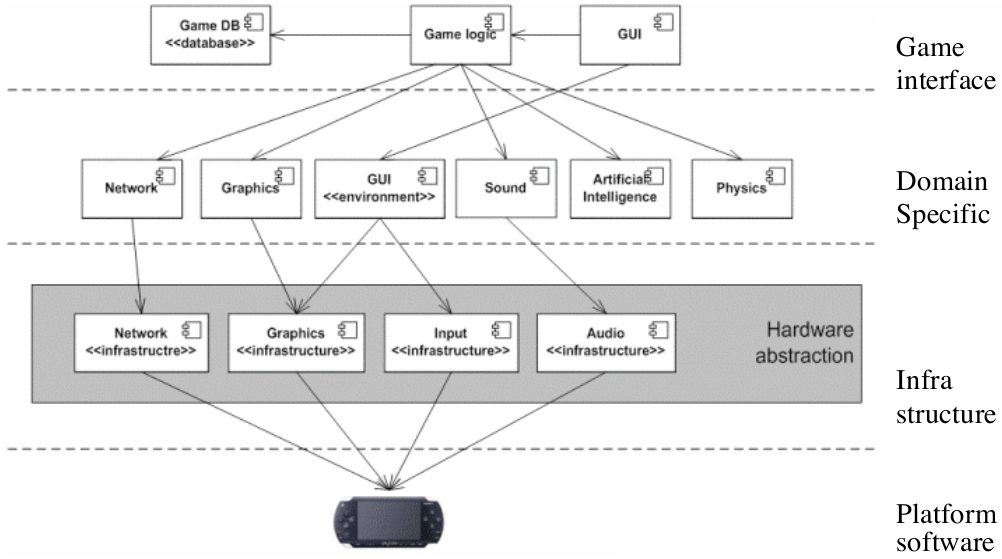
\includegraphics[scale=0.3]{pics/referencearch}
\caption{The reference architecture for games as given by Folmer -- graphic taken from the paper.}
\label{fig:referencearch}
\end{figure}

\cite{Rollings.2003} emphasizes the need for well thought-out interfaces between the components. So that for example a
route finding library/class can easily be exchanged for another one. Thus avoiding tight coupling between the high
level components where possible. He does not go into any deep details concerning components on the soft architecture
side, but he gives many ideas for design patters that can be used in game programming, such as the \textit{Singleton},
\textit{Factory} or \textit{Delegate} patters.
\linebreak

I found \citet{Fh02ageneric} particularly interesting, as it describes a system based only on components in great
detail. Haller not only explains the use of components, but also gives a very detailed proposition on how to handle
inter-component communication using a message system, based on and extending the QT GUI Framework\footnote{QT website:
\url{http://qt.nokia.com/}}.

Haller explains that components can be connected to each other using strictly typed in and outputs, making it possible to connect components
using an external (graphical) tool, easily usable by non-programmers. Having well defined in and outputs allows the
creation of component networks where as set of components are connected with each other over their in and
outputs. These networks can be looked at as a "meta-component" as the network has well defined in and outputs and can
thus itself be viewed as a component. Each component has a state in which it is in, when this state is changed a message
is sent through the outputs. The basic interface is given in \figref{fig:component}.

\begin{figure}[!htb]
\center
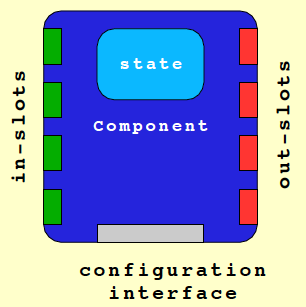
\includegraphics[scale=0.4]{pics/component}
\caption{The component interface as described by Haller \cite{Fh02ageneric} -- graphic taken from the paper.}
\label{fig:component}
\end{figure}

\cite{Doherty_2003} gives recommendations on how to structure a complete game-engine. He discusses the options of using
a component-based approach or a object-oriented design. He claimes one important advantage of using a component-based approach is:
\begin{quote}
It enforces a data-driven design philosophy. Since objects cannot be anything but data, all behavior must
be defined in terms of data. -- \cite[Page 4]{Doherty_2003}
\end{quote}
He argues this should be a favorable goal in the programming of a game, as it seperates the data from the code. By doing this it
ensures that game-designes can work in parallel with the programmers, but no recompiling of the software is needed to
change basic game attributes. Thus the teams productivity is improved.

He also brings arguments that favor the object-oriented system:
\begin{quote}
The internal representation matches the way that people think about the world. -- \cite[Page 4]{Doherty_2003}
\end{quote}

From reading his paper, I think he clearly favors the component-based approach. While acknoledging that it is more
difficult for the programmer to implement, it gives great benefitis for the game-designer. He claims that many problems
occuring with component-based systems can be solved using database proven concepts.



\subsection{Used Technology and Software}
In this section I present an overview over the technology used for this project.

\paragraph{YAML}
\begin{quote}
\textit{YAML is a human friendly data serialization standard for all programming languages.} -- \url{http://www.yaml.org}
\end{quote}
YAML has many similarities to Python, as it depends on the indention to be correct in order for the parser to work
correctly and uses a similar syntax for lists and dictionaries. This has already proven useful for the \UH{} code-base
in my experience, as all code is well formatted. These strict formatting rules should result in nicely formatted object
files and result in easier maintenance.

YAML is already being used by \UH{} to describe scenarios and campaigns, therefore it is an obvious option to use for
similar purposes.

The reason to choose YAML at the time was, that it is very easy to read and edit by humans. This comes at the cost of
being a little slower when parsing. As most data can be cached and has to be loaded from disc only once, this is not a
major concern.

\paragraph{SQLite}
\begin{quote}
\textit{SQLite is a software library that implements a self-contained, serverless, zero-configuration, transactional SQL
database engine. SQLite is the most widely deployed SQL database engine in the world. The source code for SQLite is in
the public domain.} -- \url{http://www.sqlite.org}
\end{quote}

The \UH{} project currently uses SQLite database files to store all game data, like object attributes, maps and
savegames. SQLite provides a very fast access to this data, making it a good choice where big amounts of data have to
accessed in a short amount of time -- for example map loading.

\subsubsection{Games}
In this subsection I introduce the games analyzed in this project.

\paragraph{Unknown Horizons}
\begin{quote}
\begin{center}
\includegraphics[scale=0.2]{pics/uhlogo}\end{center}
\textit{"\UH{} is a 2D realtime strategy simulation with an emphasis on economy and city building. Expand your small settlement
to a strong and wealthy colony, collect taxes and supply your inhabitants with valuable goods. Increase your power with
a well balanced economy and with strategic trade and diplomacy."} -- from \url{http://www.unknown-horizons.org}
\end{quote}

The basic game play is well known from the successful "Anno" series by Sunflowers/Ubisoft\footnote{Anno Series on
Wikipedia: \url{http://en.wikipedia.org/wiki/Category:Anno_series}}: using only few resources on a ship the player sets
out to conquer new land on an island of his choice and tries to guide his colony to wealth and power.

\UH{} has been been in active development for over four years and has been played by many thousands players from around
the world\footnote{\UH{} download statistics: \url{http://sourceforge.net/projects/unknownhorizons/files/Unknown
Horizons/}}. 

This year (2011) \UH{} participated in the \textit{Google Summer of Code} mentoring three successful students
together with its graphics engine FIFE\footnote{FIFE website: \url{http://www.fifengine.net}}, demonstrating that it has
an active community and is regarded as an important part of the \OS{} gaming world.

\paragraph{The Battle of Wesnoth}
\begin{quote}
\begin{center}
\includegraphics[scale=0.4]{pics/wesnothlogo}\end{center}
\textit{"The Battle for Wesnoth is a Free, turn-based tactical strategy game with a high fantasy theme, featuring both
single-player, and online/hotseat multiplayer combat. Fight a desperate battle to reclaim the throne of Wesnoth, or take
hand in any number of other adventures..."} -- from \url{http://www.wesnoth.org}
\end{quote}

\BOW{} is probably one of the best known and most stable \OS{} games on the market and has a huge developer community
with 103 registered developers on their GNA project page\footnote{\BOW{} gna.org page:
\url{http://gna.org/projects/wesnoth/}} and approaching ticket number 20000 on their bugtracker\footnote{\BOW{}
bugtracker: \url{http://gna.org/bugs/?group=wesnoth}}. Over 20000 members are registered at the project's forum:
\url{http://forums.wesnoth.org/}.

The first released version was 0.1 in 2003, version 1.0 was released in 2006. The current stable release 1.8.6 has over
190.000 downloads on sourceforge\footnote{\BOW{} downloads page:
\url{http://sourceforge.net/projects/wesnoth/files/wesnoth-1.8/}}. With the mature state of the project it makes for
an interesting case-study candidate.

\paragraph{MegaGlest}
\begin{quote}
\begin{center}
\includegraphics[scale=0.5]{pics/glestlogo}\end{center}
\textit{"MegaGlest is a free and open source 3D real-time strategy (RTS) game, where you control the armies of one of
seven different factions: Tech, Magic, Egyptians, Indians, Norsemen, Persian or Romans. The game is setup in one of 16
naturally looking settings, which -like the unit models- are crafted with great appreciation for detail. Additional game
data can be downloaded from within the game at no cost."} -- from \url{http://www.megaglest.org}
\end{quote}

\GLEST{} is a fork of the old project \textit{GLEST} on which development has stopped. \textit{GLEST} is now being
developed in two versions \GLEST{} and \textit{Glest Advanced Engine}. \GLEST{} is the stabler version of these two
projects which is why I chose to analyze it instead of the \textit{Glest Advanced Engine}.

\textit{GLEST} version 1.0.0 was released in 2004, the first \GLEST{} version (3.3.2) was released in
2010\footnote{\GLEST 3.3.2 release announcement: \url{http://glest.org/glest_board/index.php?topic=4917.0}}. With it's
long history \GLEST{} is a very mature game with a big community, making it a good choice for my case-study.

\paragraph{0A.D.}
\begin{quote}
\begin{center}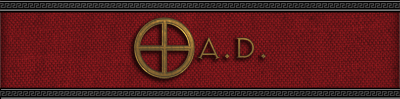
\includegraphics[scale=0.8]{pics/0ad}\end{center}
\textit{"0 A.D. (pronounced “zero ey-dee”) is a free, open-source, cross-platform real-time strategy (RTS) game of
ancient warfare. In short, it is a historically-based war/economy game that allows players to relive or rewrite the
history of Western civilizations, focusing on the years between 500 B.C. and 500 A.D. The project is highly ambitious,
involving state-of-the-art 3D graphics, detailed artwork, sound, and a flexible and powerful custom-built game engine."}
-- from \url{http://wildfiregames.com/0ad/}
\end{quote}

\AD{} started as a total conversion for \textit{Age of Empires II} by a group of friends. The team quickly moved to
their own game concept as they felt limited in their possibilities by the idea of a total conversion. The code was made
\OS{} only in 2009, the first releases followed in 2010.

The fact that the developers explicitly try to develop a engine and a game, not both in one should provide interesting
insight on the design decisions necessary when creating a game-engine.





